\documentclass[12pt,a4paper]{article}

\usepackage[a4paper,text={16.5cm,25.2cm},centering]{geometry}
\usepackage{lmodern}
\usepackage{amssymb,amsmath}
\usepackage{bm}
\usepackage{graphicx}
\usepackage{microtype}
\usepackage{hyperref}
\setlength{\parindent}{0pt}
\setlength{\parskip}{1.2ex}

\hypersetup
       {   pdfauthor = { Sheehan Olver },
           pdftitle={ foo },
           colorlinks=TRUE,
           linkcolor=black,
           citecolor=blue,
           urlcolor=blue
       }




\usepackage{upquote}
\usepackage{listings}
\usepackage{xcolor}
\lstset{
    basicstyle=\ttfamily\footnotesize,
    upquote=true,
    breaklines=true,
    breakindent=0pt,
    keepspaces=true,
    showspaces=false,
    columns=fullflexible,
    showtabs=false,
    showstringspaces=false,
    escapeinside={(*@}{@*)},
    extendedchars=true,
}
\newcommand{\HLJLt}[1]{#1}
\newcommand{\HLJLw}[1]{#1}
\newcommand{\HLJLe}[1]{#1}
\newcommand{\HLJLeB}[1]{#1}
\newcommand{\HLJLo}[1]{#1}
\newcommand{\HLJLk}[1]{\textcolor[RGB]{148,91,176}{\textbf{#1}}}
\newcommand{\HLJLkc}[1]{\textcolor[RGB]{59,151,46}{\textit{#1}}}
\newcommand{\HLJLkd}[1]{\textcolor[RGB]{214,102,97}{\textit{#1}}}
\newcommand{\HLJLkn}[1]{\textcolor[RGB]{148,91,176}{\textbf{#1}}}
\newcommand{\HLJLkp}[1]{\textcolor[RGB]{148,91,176}{\textbf{#1}}}
\newcommand{\HLJLkr}[1]{\textcolor[RGB]{148,91,176}{\textbf{#1}}}
\newcommand{\HLJLkt}[1]{\textcolor[RGB]{148,91,176}{\textbf{#1}}}
\newcommand{\HLJLn}[1]{#1}
\newcommand{\HLJLna}[1]{#1}
\newcommand{\HLJLnb}[1]{#1}
\newcommand{\HLJLnbp}[1]{#1}
\newcommand{\HLJLnc}[1]{#1}
\newcommand{\HLJLncB}[1]{#1}
\newcommand{\HLJLnd}[1]{\textcolor[RGB]{214,102,97}{#1}}
\newcommand{\HLJLne}[1]{#1}
\newcommand{\HLJLneB}[1]{#1}
\newcommand{\HLJLnf}[1]{\textcolor[RGB]{66,102,213}{#1}}
\newcommand{\HLJLnfm}[1]{\textcolor[RGB]{66,102,213}{#1}}
\newcommand{\HLJLnp}[1]{#1}
\newcommand{\HLJLnl}[1]{#1}
\newcommand{\HLJLnn}[1]{#1}
\newcommand{\HLJLno}[1]{#1}
\newcommand{\HLJLnt}[1]{#1}
\newcommand{\HLJLnv}[1]{#1}
\newcommand{\HLJLnvc}[1]{#1}
\newcommand{\HLJLnvg}[1]{#1}
\newcommand{\HLJLnvi}[1]{#1}
\newcommand{\HLJLnvm}[1]{#1}
\newcommand{\HLJLl}[1]{#1}
\newcommand{\HLJLld}[1]{\textcolor[RGB]{148,91,176}{\textit{#1}}}
\newcommand{\HLJLs}[1]{\textcolor[RGB]{201,61,57}{#1}}
\newcommand{\HLJLsa}[1]{\textcolor[RGB]{201,61,57}{#1}}
\newcommand{\HLJLsb}[1]{\textcolor[RGB]{201,61,57}{#1}}
\newcommand{\HLJLsc}[1]{\textcolor[RGB]{201,61,57}{#1}}
\newcommand{\HLJLsd}[1]{\textcolor[RGB]{201,61,57}{#1}}
\newcommand{\HLJLsdB}[1]{\textcolor[RGB]{201,61,57}{#1}}
\newcommand{\HLJLsdC}[1]{\textcolor[RGB]{201,61,57}{#1}}
\newcommand{\HLJLse}[1]{\textcolor[RGB]{59,151,46}{#1}}
\newcommand{\HLJLsh}[1]{\textcolor[RGB]{201,61,57}{#1}}
\newcommand{\HLJLsi}[1]{#1}
\newcommand{\HLJLso}[1]{\textcolor[RGB]{201,61,57}{#1}}
\newcommand{\HLJLsr}[1]{\textcolor[RGB]{201,61,57}{#1}}
\newcommand{\HLJLss}[1]{\textcolor[RGB]{201,61,57}{#1}}
\newcommand{\HLJLssB}[1]{\textcolor[RGB]{201,61,57}{#1}}
\newcommand{\HLJLnB}[1]{\textcolor[RGB]{59,151,46}{#1}}
\newcommand{\HLJLnbB}[1]{\textcolor[RGB]{59,151,46}{#1}}
\newcommand{\HLJLnfB}[1]{\textcolor[RGB]{59,151,46}{#1}}
\newcommand{\HLJLnh}[1]{\textcolor[RGB]{59,151,46}{#1}}
\newcommand{\HLJLni}[1]{\textcolor[RGB]{59,151,46}{#1}}
\newcommand{\HLJLnil}[1]{\textcolor[RGB]{59,151,46}{#1}}
\newcommand{\HLJLnoB}[1]{\textcolor[RGB]{59,151,46}{#1}}
\newcommand{\HLJLoB}[1]{\textcolor[RGB]{102,102,102}{\textbf{#1}}}
\newcommand{\HLJLow}[1]{\textcolor[RGB]{102,102,102}{\textbf{#1}}}
\newcommand{\HLJLp}[1]{#1}
\newcommand{\HLJLc}[1]{\textcolor[RGB]{153,153,119}{\textit{#1}}}
\newcommand{\HLJLch}[1]{\textcolor[RGB]{153,153,119}{\textit{#1}}}
\newcommand{\HLJLcm}[1]{\textcolor[RGB]{153,153,119}{\textit{#1}}}
\newcommand{\HLJLcp}[1]{\textcolor[RGB]{153,153,119}{\textit{#1}}}
\newcommand{\HLJLcpB}[1]{\textcolor[RGB]{153,153,119}{\textit{#1}}}
\newcommand{\HLJLcs}[1]{\textcolor[RGB]{153,153,119}{\textit{#1}}}
\newcommand{\HLJLcsB}[1]{\textcolor[RGB]{153,153,119}{\textit{#1}}}
\newcommand{\HLJLg}[1]{#1}
\newcommand{\HLJLgd}[1]{#1}
\newcommand{\HLJLge}[1]{#1}
\newcommand{\HLJLgeB}[1]{#1}
\newcommand{\HLJLgh}[1]{#1}
\newcommand{\HLJLgi}[1]{#1}
\newcommand{\HLJLgo}[1]{#1}
\newcommand{\HLJLgp}[1]{#1}
\newcommand{\HLJLgs}[1]{#1}
\newcommand{\HLJLgsB}[1]{#1}
\newcommand{\HLJLgt}[1]{#1}



\def\qqand{\qquad\hbox{and}\qquad}
\def\qqfor{\qquad\hbox{for}\qquad}
\def\D{ {\rm d} }
\def\I{ {\rm i} }
\def\E{ {\rm e} }
\def\C{ {\mathbb C} }
\def\R{ {\mathbb R} }
\def\CC{ {\cal C} }
\def\HH{ {\cal H} }
\def\vc#1{ {\mathbf #1} }
\def\bbC{ {\mathbb C} }

\def\qqqquad{\qquad\qquad}
\def\qqfor{\qquad\hbox{for}\qquad}
\def\qqwhere{\qquad\hbox{where}\qquad}
\def\Res_#1{\underset{#1}{\rm Res}\,}
\def\sech{ {\rm sech}\, }



\def\Xint#1{ \mathchoice
   {\XXint\displaystyle\textstyle{#1} }%
   {\XXint\textstyle\scriptstyle{#1} }%
   {\XXint\scriptstyle\scriptscriptstyle{#1} }%
   {\XXint\scriptscriptstyle\scriptscriptstyle{#1} }%
   \!\int}
\def\XXint#1#2#3{ {\setbox0=\hbox{$#1{#2#3}{\int}$}
     \vcenter{\hbox{$#2#3$}}\kern-.5\wd0} }
\def\ddashint{\Xint=}
\def\dashint{\Xint-}
% \def\dashint
\def\infdashint{\dashint_{-\infty}^\infty}




\def\addtab#1={#1\;&=}
\def\ccr{\\\addtab}
\def\ip<#1>{\left\langle{#1}\right\rangle}
\def\dx{\D x}
\def\dt{\D t}
\def\dz{\D z}

\def\norm#1{\left\| #1 \right\|}

\def\pr(#1){\left({#1}\right)}
\def\br[#1]{\left[{#1}\right]}

\def\abs#1{\left|{#1}\right|}
\def\fpr(#1){\!\pr({#1})}

\def\sopmatrix#1{ \begin{pmatrix}#1\end{pmatrix} }

\def\endash{–}
\def\mdblksquare{\blacksquare}

\begin{document}

\textbf{M3M6: Methods of Mathematical Physics}

Dr. Sheehan Olver

s.olver@imperial.ac.uk

\section{Lecture 4: Applications to real integrals}
This lecture we discuss applications of residue calculus. 

\begin{itemize}
\item[1. ] Trigonometric integrals


\item[2. ] Integrals over real lines

\begin{itemize}
\item Principal value integral


\item Cauchy's integral formula and Residue theorem on the real line

\end{itemize}

\item[3. ] Oscillatory integrals

\begin{itemize}
\item Jordan's lemma


\item Application: Calculating Fourier tranforms of weakly decaying functions

\end{itemize}
\end{itemize}
\subsection{Trigonomteric}
We can calculate integrals of the form 

\[
\int_0^{2 \pi} R(\cos \theta, \sin \theta) \D \theta
\]
where $R(x,y)$ is rational by doing the change of variables $z = e^{\I \theta}$ to reduce it to

\[
\oint_{C_1} R\left({z + z^{-1} \over 2}, {z - z^{-1} \over 2 \I} \right) {\D z \over \I z}
\]
This is rational in $z$ hence guaranteed to be amenable to residue calculus, provided we can find the poles of the denominator. 

\emph{Example} Consider

\[
\int_0^{2\pi} {\D \theta \over 1 - 2\rho \cos \theta + \rho^2}
\]
for $0 < \rho < 1$. We need to first locate the poles of 

\[
f(z)= R\left({z + z^{-1} \over 2}, {z - z^{-1} \over 2 \I} \right) {1 \over \I z} = 
{ \I \over \rho z^2 - (1+\rho^2) z + \rho}
\]
This has poles at 

\[
z = {1 + \rho^2 \pm \sqrt{(1+\rho^2)^2 - 4 \rho^2 } \over 2} = \rho, \rho^{-1}
\]
We can confirm this with a phase plot:


\begin{lstlisting}
(*@\HLJLk{using}@*) (*@\HLJLn{Plots}@*)(*@\HLJLp{,}@*) (*@\HLJLn{ComplexPhasePortrait}@*)
(*@\HLJLn{\ensuremath{\rho}}@*) (*@\HLJLoB{=}@*) (*@\HLJLnfB{0.5}@*)
(*@\HLJLnf{phaseplot}@*)(*@\HLJLp{(}@*)(*@\HLJLoB{-}@*)(*@\HLJLnfB{2..2}@*)(*@\HLJLp{,}@*) (*@\HLJLoB{-}@*)(*@\HLJLnfB{2..2}@*)(*@\HLJLp{,}@*) (*@\HLJLn{z}@*) (*@\HLJLoB{->}@*)  (*@\HLJLni{1}@*)(*@\HLJLoB{/}@*)(*@\HLJLp{(}@*)(*@\HLJLni{1}@*)(*@\HLJLoB{-}@*)(*@\HLJLn{\ensuremath{\rho}}@*)(*@\HLJLoB{*}@*)(*@\HLJLp{(}@*)(*@\HLJLn{z}@*)(*@\HLJLoB{+}@*)(*@\HLJLp{(}@*)(*@\HLJLn{z}@*)(*@\HLJLoB{{\textasciicircum}}@*)(*@\HLJLp{(}@*)(*@\HLJLoB{-}@*)(*@\HLJLni{1}@*)(*@\HLJLp{)))}@*) (*@\HLJLoB{+}@*) (*@\HLJLn{\ensuremath{\rho}}@*)(*@\HLJLoB{{\textasciicircum}}@*)(*@\HLJLni{2}@*)(*@\HLJLp{)}@*) (*@\HLJLoB{*}@*) (*@\HLJLni{1}@*)(*@\HLJLoB{/}@*)(*@\HLJLp{(}@*)(*@\HLJLn{im}@*)(*@\HLJLoB{*}@*)(*@\HLJLn{z}@*)(*@\HLJLp{))}@*)
\end{lstlisting}

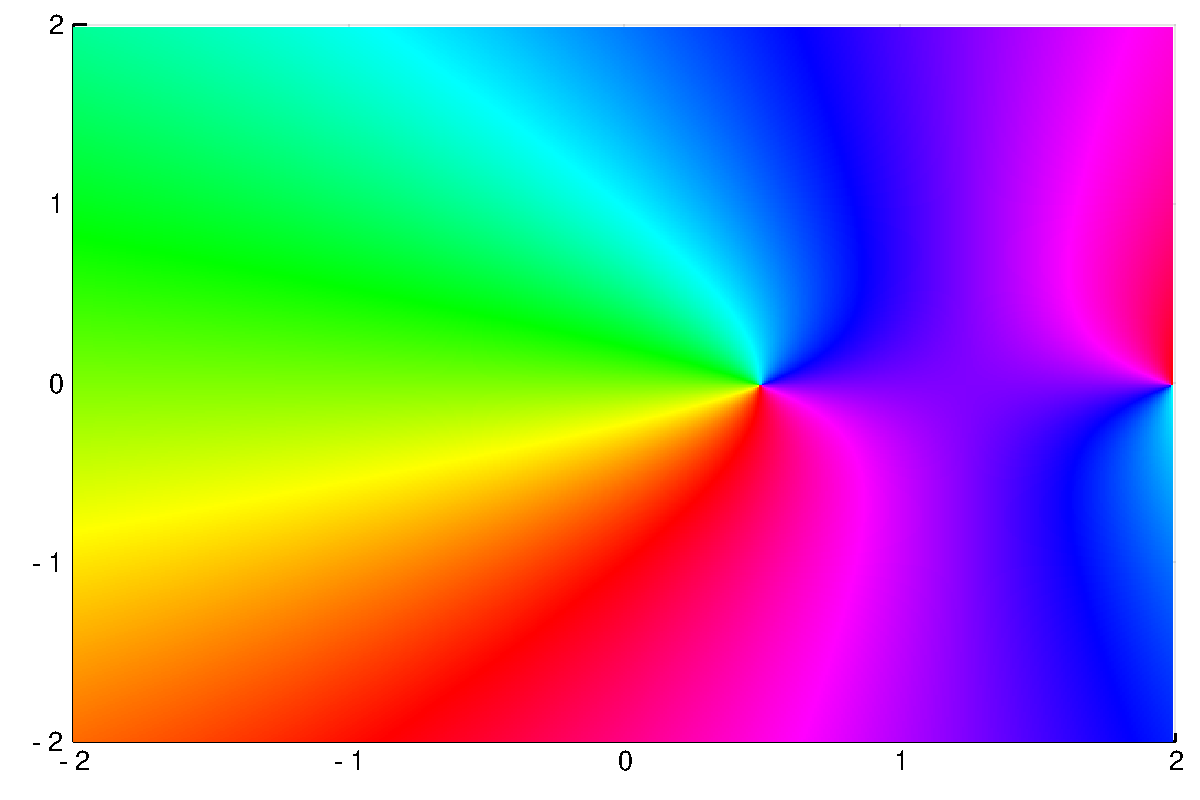
\includegraphics[width=\linewidth]{figures/Lecture5_1_1.pdf}

Thus we can use either the interior or exterior residue calculus.  Since we know then roots of the denominator of $f$ we determine that

\[
f(z) = {\I \over (z - \rho) (\rho z - 1)}
\]
Thus we find

\[
\int_0^{2\pi} {\D \theta \over 1 - 2\rho \cos \theta + \rho^2} = 2 \pi \I \Res_{z = \rho} f(z) = 
-2 \pi \I \Res_{z = 1/\rho} f(z) = {2 \pi \over 1 - \rho^2}.
\]
\subsection{Integrals over the real line}
Integrals on the real line are typically viewed as improper integrals:

\[
\int_{-\infty}^\infty f(x) \dx = \int_0^\infty f(x) \dx +\int_{-\infty}^0 f(x)\dx = 
\lim_{b \rightarrow \infty} \int_0^b f(x) \dx + \lim_{a \rightarrow -\infty} \int_a^0 f(x) \dx.
\]
It is convenient to work with a slightly different notion where we take the limit simealtaneously:

\textbf{Definition (Principal value integral on the real line)} The \emph{(Cauchy) principal value integral on the real line} is defined as

\[
\infdashint f(x) \dx := \lim_{M\rightarrow \infty} \int_{-M}^M f(x) \dx
\]
This is a weaker concept:

\textbf{Proposition (Integability $\Rightarrow$ Prinipal value integrability)} If  $\int_{-\infty}^\infty f(x) \dx < \infty$ then 

\[
\infdashint f(x) \dx = \int_{-\infty}^\infty f(x) \dx.
\]
\textbf{Example} Consider integrating $1/(x-\I)$ with indefinite integral $\log(x-\I)$. We use the Definition

\[
\log z = \log |z| + \I \arg z
\]
where $- \pi \leq \arg z < \pi$. Thus we have


\begin{align*}
\lim_{b \rightarrow \infty} \log(b - \I) = \lim_{b \rightarrow \infty} \log|b - \I| = \infty \\
\lim_{a \rightarrow -\infty} \log(a - \I) = \lim_{a \rightarrow -\infty} (\log|a - \I| + \I \arg(a-\I)) = \infty - \pi \I 
\end{align*}
Thus

\[
\int_{-\infty}^\infty {\dx \over x - \I} = \lim_{a \rightarrow -\infty} \br[\log(-\I) - \log(a-\I)] + 
\lim_{b \rightarrow \infty} \br[\log(b-\I) - \log(-\I)] =  -\infty + \I \pi + \infty
\]
is undefined. On the other hand, the Cauchy principal value integral gives

\[
\infdashint {\dx \over x - \I} = \lim_{M \rightarrow \infty} \br[\log(M-\I) - \log(-M - \I)] =
 \lim_{M \rightarrow \infty} \br[\log|M-\I| - \log|-M - \I|]  + \I \pi = \I \pi.
\]
\subsubsection{Residue theorem on the real line}
The real line doesn't have an \emph{inside} and \emph{outside}, rather an \emph{above} and \emph{below}, or \emph{left} and \emph{right}. Thus we get the following two versions of the Residue theorem:

\textbf{Definition (Upper/lower half plane)} Denote the upper/lower half plane by


\begin{align*}
{\mathbb H}^+ = \{z : \Re z > 0 \}  \\
{\mathbb H}^- = \{z : \Re z < 0 \} 
\end{align*}
The closure is denoted


\begin{align*}
\bar{\mathbb H}^+ = {\mathbb H}^+ \cup {\mathbb R} \cup \{\infty\}  \\
\bar{\mathbb H}^- = {\mathbb H}^- \cup {\mathbb R} \cup \{\infty\}
\end{align*}
\textbf{Theorem (Residue theorem on the real line)} Suppose $f : \bar {\mathbb H}^+ \backslash \{z_1,\ldots,z_r \} \rightarrow {\mathbb C}$ is holomorphic in ${\mathbb H}^+ \backslash \{z_1,\ldots,z_r \}$, where $\Re z_k > 0$, and  $\lim_{\epsilon \rightarrow 0} f(x + i \epsilon) = f(x)$ converges uniformly.  If 

\[
\lim_{z \rightarrow \infty} z f(z) = 0
\]
uniformly for $z \in \bar {\mathbb H}^+$, then

\[
\infdashint f(x) \dx = 2 \pi \I \sum_{k=1}^r {\underset{z = z_k}{\rm Res}} \, f(z)
\]
Similarly, if the equivalent conditions hold in the lower half plane for $f : \bar{\mathbb H}^- \backslash \{z_1,\ldots,z_r \} \rightarrow {\mathbb C}$ then

\[
\infdashint f(x) \dx = -2 \pi \I \sum_{k=1}^r {\underset{z = z_k}{\rm Res}} \, f(z)
\]
\textbf{Proof}  This follows by considering  the contour $\gamma_R = [-R,R] \cup H_R$ where 

\[
H_R := \{ R \E^{\I \theta} : 0 \leq \theta \leq \pi \},
\]
that is, the upper-half circle. Classical residue calculus gives

\[
\oint_{\gamma_R} f(z) \dz =  2\pi \I \sum_{k=1}^r {\underset{z = z_k}{\rm Res}} \, f(z).
\]
provided $R$ is large enough to contain all singularities. But the decay in $f$ suffices to show that $\int_{H_R} f(z) \D z \rightarrow 0$ as $R \rightarrow \infty$.  The result therefore follows.

\ensuremath{\blacksquare}

\emph{Demonstration}


\begin{lstlisting}
(*@\HLJLn{f}@*) (*@\HLJLoB{=}@*) (*@\HLJLn{x}@*) (*@\HLJLoB{->}@*) (*@\HLJLn{x}@*)(*@\HLJLoB{{\textasciicircum}}@*)(*@\HLJLni{2}@*)(*@\HLJLoB{/}@*)(*@\HLJLp{(}@*)(*@\HLJLn{x}@*)(*@\HLJLoB{{\textasciicircum}}@*)(*@\HLJLni{4}@*)(*@\HLJLoB{+}@*)(*@\HLJLni{1}@*)(*@\HLJLp{)}@*)
(*@\HLJLnf{phaseplot}@*)(*@\HLJLp{(}@*)(*@\HLJLoB{-}@*)(*@\HLJLnfB{3..3}@*)(*@\HLJLp{,}@*) (*@\HLJLoB{-}@*)(*@\HLJLnfB{2..2}@*)(*@\HLJLp{,}@*) (*@\HLJLn{f}@*)(*@\HLJLp{)}@*)
\end{lstlisting}

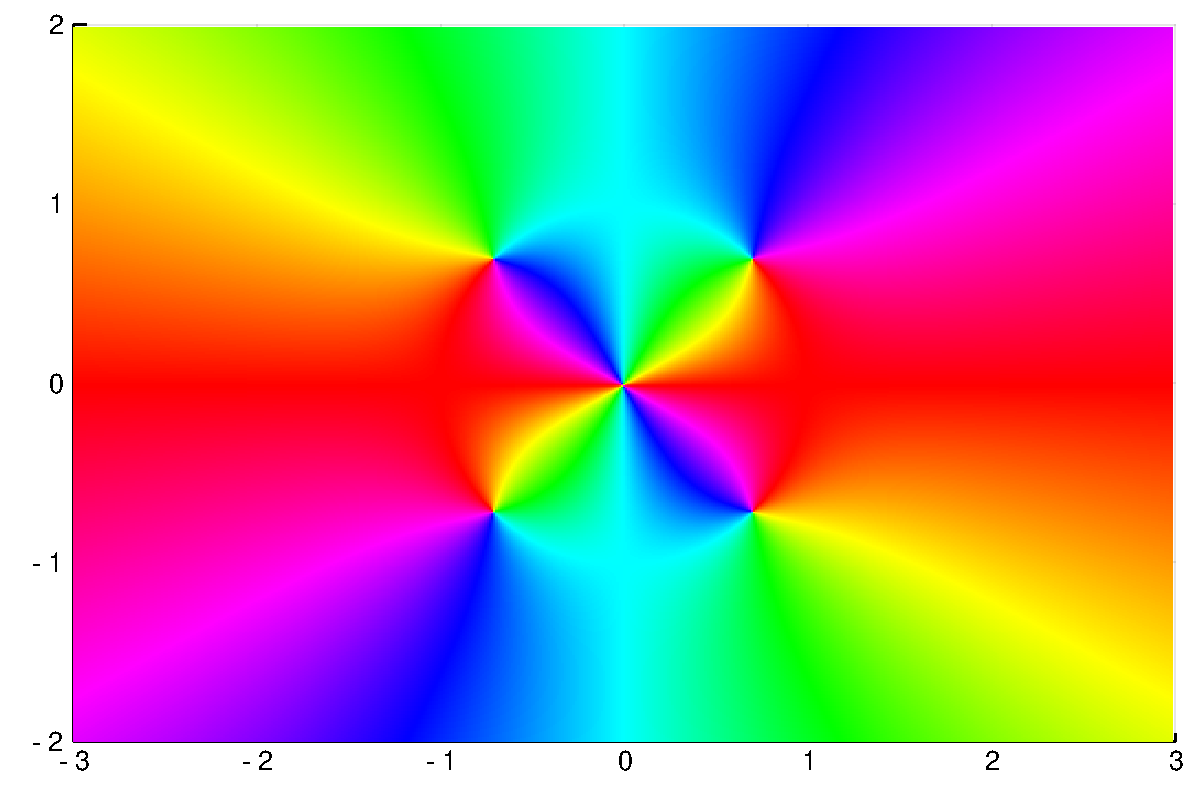
\includegraphics[width=\linewidth]{figures/Lecture5_2_1.pdf}

This function has poles in the upper plane, but has sufficient decay that we can apply Residue theorem:


\begin{lstlisting}
(*@\HLJLk{using}@*) (*@\HLJLn{ApproxFun}@*)
(*@\HLJLn{z\ensuremath{\_1}}@*)(*@\HLJLp{,}@*)(*@\HLJLn{z\ensuremath{\_2}}@*)(*@\HLJLp{,}@*)(*@\HLJLn{z\ensuremath{\_3}}@*)(*@\HLJLp{,}@*)(*@\HLJLn{z\ensuremath{\_4}}@*) (*@\HLJLoB{=}@*) (*@\HLJLnf{exp}@*)(*@\HLJLp{(}@*)(*@\HLJLn{im}@*)(*@\HLJLoB{*}@*)(*@\HLJLn{\ensuremath{\pi}}@*)(*@\HLJLoB{/}@*)(*@\HLJLni{4}@*)(*@\HLJLp{),}@*) (*@\HLJLnf{exp}@*)(*@\HLJLp{(}@*)(*@\HLJLni{3}@*)(*@\HLJLn{im}@*)(*@\HLJLoB{*}@*)(*@\HLJLn{\ensuremath{\pi}}@*)(*@\HLJLoB{/}@*)(*@\HLJLni{4}@*)(*@\HLJLp{),}@*) (*@\HLJLnf{exp}@*)(*@\HLJLp{(}@*)(*@\HLJLni{5}@*)(*@\HLJLn{im}@*)(*@\HLJLoB{*}@*)(*@\HLJLn{\ensuremath{\pi}}@*)(*@\HLJLoB{/}@*)(*@\HLJLni{4}@*)(*@\HLJLp{),}@*) (*@\HLJLnf{exp}@*)(*@\HLJLp{(}@*)(*@\HLJLni{7}@*)(*@\HLJLn{im}@*)(*@\HLJLoB{*}@*)(*@\HLJLn{\ensuremath{\pi}}@*)(*@\HLJLoB{/}@*)(*@\HLJLni{4}@*)(*@\HLJLp{)}@*)

(*@\HLJLn{res\ensuremath{\_1}}@*) (*@\HLJLoB{=}@*) (*@\HLJLn{z\ensuremath{\_1}}@*)(*@\HLJLoB{{\textasciicircum}}@*)(*@\HLJLni{2}@*) (*@\HLJLoB{/}@*) (*@\HLJLp{((}@*)(*@\HLJLn{z\ensuremath{\_1}}@*) (*@\HLJLoB{-}@*) (*@\HLJLn{z\ensuremath{\_2}}@*)(*@\HLJLp{)}@*)(*@\HLJLoB{*}@*)(*@\HLJLp{(}@*)(*@\HLJLn{z\ensuremath{\_1}}@*) (*@\HLJLoB{-}@*) (*@\HLJLn{z\ensuremath{\_3}}@*)(*@\HLJLp{)}@*)(*@\HLJLoB{*}@*)(*@\HLJLp{(}@*)(*@\HLJLn{z\ensuremath{\_1}}@*) (*@\HLJLoB{-}@*) (*@\HLJLn{z\ensuremath{\_4}}@*)(*@\HLJLp{)}@*) (*@\HLJLp{)}@*)
(*@\HLJLn{res\ensuremath{\_2}}@*) (*@\HLJLoB{=}@*) (*@\HLJLn{z\ensuremath{\_2}}@*)(*@\HLJLoB{{\textasciicircum}}@*)(*@\HLJLni{2}@*) (*@\HLJLoB{/}@*) (*@\HLJLp{((}@*)(*@\HLJLn{z\ensuremath{\_2}}@*) (*@\HLJLoB{-}@*) (*@\HLJLn{z\ensuremath{\_1}}@*)(*@\HLJLp{)}@*)(*@\HLJLoB{*}@*)(*@\HLJLp{(}@*)(*@\HLJLn{z\ensuremath{\_2}}@*) (*@\HLJLoB{-}@*) (*@\HLJLn{z\ensuremath{\_3}}@*)(*@\HLJLp{)}@*)(*@\HLJLoB{*}@*)(*@\HLJLp{(}@*)(*@\HLJLn{z\ensuremath{\_2}}@*) (*@\HLJLoB{-}@*) (*@\HLJLn{z\ensuremath{\_4}}@*)(*@\HLJLp{)}@*) (*@\HLJLp{)}@*)

(*@\HLJLni{2}@*)(*@\HLJLn{\ensuremath{\pi}}@*)(*@\HLJLoB{*}@*)(*@\HLJLn{im}@*)(*@\HLJLoB{*}@*)(*@\HLJLp{(}@*)(*@\HLJLn{res\ensuremath{\_1}}@*) (*@\HLJLoB{+}@*) (*@\HLJLn{res\ensuremath{\_2}}@*)(*@\HLJLp{),}@*) (*@\HLJLnf{sum}@*)(*@\HLJLp{(}@*)(*@\HLJLnf{Fun}@*)(*@\HLJLp{(}@*)(*@\HLJLn{f}@*)(*@\HLJLp{,}@*) (*@\HLJLnf{Line}@*)(*@\HLJLp{()))}@*)
\end{lstlisting}

\begin{lstlisting}
(2.221441469079183 + 3.487868498008632e-16im, 2.221441469084968)
\end{lstlisting}


We can also apply Resiude theorem in the lower-half plane, and we get the same result:


\begin{lstlisting}
(*@\HLJLn{res\ensuremath{\_3}}@*) (*@\HLJLoB{=}@*) (*@\HLJLn{z\ensuremath{\_3}}@*)(*@\HLJLoB{{\textasciicircum}}@*)(*@\HLJLni{2}@*) (*@\HLJLoB{/}@*) (*@\HLJLp{((}@*)(*@\HLJLn{z\ensuremath{\_3}}@*) (*@\HLJLoB{-}@*) (*@\HLJLn{z\ensuremath{\_1}}@*)(*@\HLJLp{)}@*)(*@\HLJLoB{*}@*)(*@\HLJLp{(}@*)(*@\HLJLn{z\ensuremath{\_3}}@*) (*@\HLJLoB{-}@*) (*@\HLJLn{z\ensuremath{\_2}}@*)(*@\HLJLp{)}@*)(*@\HLJLoB{*}@*)(*@\HLJLp{(}@*)(*@\HLJLn{z\ensuremath{\_3}}@*) (*@\HLJLoB{-}@*) (*@\HLJLn{z\ensuremath{\_4}}@*)(*@\HLJLp{)}@*) (*@\HLJLp{)}@*)
(*@\HLJLn{res\ensuremath{\_4}}@*) (*@\HLJLoB{=}@*) (*@\HLJLn{z\ensuremath{\_4}}@*)(*@\HLJLoB{{\textasciicircum}}@*)(*@\HLJLni{2}@*) (*@\HLJLoB{/}@*) (*@\HLJLp{((}@*)(*@\HLJLn{z\ensuremath{\_4}}@*) (*@\HLJLoB{-}@*) (*@\HLJLn{z\ensuremath{\_1}}@*)(*@\HLJLp{)}@*)(*@\HLJLoB{*}@*)(*@\HLJLp{(}@*)(*@\HLJLn{z\ensuremath{\_4}}@*) (*@\HLJLoB{-}@*) (*@\HLJLn{z\ensuremath{\_3}}@*)(*@\HLJLp{)}@*)(*@\HLJLoB{*}@*)(*@\HLJLp{(}@*)(*@\HLJLn{z\ensuremath{\_4}}@*) (*@\HLJLoB{-}@*) (*@\HLJLn{z\ensuremath{\_2}}@*)(*@\HLJLp{)}@*) (*@\HLJLp{)}@*)

(*@\HLJLoB{-}@*)(*@\HLJLni{2}@*)(*@\HLJLn{\ensuremath{\pi}}@*)(*@\HLJLoB{*}@*)(*@\HLJLn{im}@*)(*@\HLJLoB{*}@*)(*@\HLJLp{(}@*)(*@\HLJLn{res\ensuremath{\_3}}@*) (*@\HLJLoB{+}@*) (*@\HLJLn{res\ensuremath{\_4}}@*)(*@\HLJLp{),}@*) (*@\HLJLnf{sum}@*)(*@\HLJLp{(}@*)(*@\HLJLnf{Fun}@*)(*@\HLJLp{(}@*)(*@\HLJLn{f}@*)(*@\HLJLp{,}@*) (*@\HLJLnf{Line}@*)(*@\HLJLp{()))}@*)
\end{lstlisting}

\begin{lstlisting}
(2.221441469079183 + 5.231802747012948e-16im, 2.221441469084968)
\end{lstlisting}


\subsubsection{Cauchy's integral formula on the real line}
An immediate consequence of the Residue theorem is Cauchy's integral formula on the real line:

\textbf{Theorem (Cauchy's integral formula on the real line)} Suppose $f : \bar {\mathbb H}^+  \rightarrow {\mathbb C}$ is holomorphic in ${\mathbb H}^+ $, and  $\lim_{\epsilon \rightarrow 0} f(x + i \epsilon) = f(x)$ converges uniformly.  If 

\[
\lim_{z \rightarrow \infty} f(z) = 0
\]
uniformly for $z \in \bar {\mathbb H}^+$, then

\[
f(z) = {1 \over 2 \pi \I} \infdashint {f(x) \over x - z} dx
\]
for all  $z \in {\mathbb H}^+$.

\emph{Examples} Here is a simple example of $f(x) = {x^2 \over (x+ i)^3}$, which is analytic in the upper half plane:


\begin{lstlisting}
(*@\HLJLn{f}@*) (*@\HLJLoB{=}@*) (*@\HLJLn{x}@*) (*@\HLJLoB{->}@*) (*@\HLJLn{x}@*)(*@\HLJLoB{{\textasciicircum}}@*)(*@\HLJLni{2}@*)(*@\HLJLoB{/}@*)(*@\HLJLp{(}@*)(*@\HLJLn{x}@*)(*@\HLJLoB{+}@*)(*@\HLJLn{im}@*)(*@\HLJLp{)}@*)(*@\HLJLoB{{\textasciicircum}}@*)(*@\HLJLni{3}@*)
(*@\HLJLn{z}@*) (*@\HLJLoB{=}@*) (*@\HLJLnfB{2.0}@*)(*@\HLJLoB{+}@*)(*@\HLJLnfB{2.0}@*)(*@\HLJLn{im}@*)
(*@\HLJLnf{sum}@*)(*@\HLJLp{(}@*)(*@\HLJLnf{Fun}@*)(*@\HLJLp{(}@*)(*@\HLJLn{x}@*)(*@\HLJLoB{->}@*) (*@\HLJLnf{f}@*)(*@\HLJLp{(}@*)(*@\HLJLn{x}@*)(*@\HLJLp{)}@*)(*@\HLJLoB{/}@*)(*@\HLJLp{(}@*)(*@\HLJLn{x}@*) (*@\HLJLoB{-}@*) (*@\HLJLn{z}@*)(*@\HLJLp{),}@*) (*@\HLJLnf{Line}@*)(*@\HLJLp{()))}@*)(*@\HLJLoB{/}@*)(*@\HLJLp{(}@*)(*@\HLJLni{2}@*)(*@\HLJLn{\ensuremath{\pi}}@*)(*@\HLJLoB{*}@*)(*@\HLJLn{im}@*)(*@\HLJLp{)}@*) (*@\HLJLoB{-}@*) (*@\HLJLnf{f}@*)(*@\HLJLp{(}@*)(*@\HLJLn{z}@*)(*@\HLJLp{)}@*)
\end{lstlisting}

\begin{lstlisting}
2.69638478211931e-13 - 3.032296636007459e-13im
\end{lstlisting}


Evaluating in lower half plane doesn't work because it has a pole there:


\begin{lstlisting}
(*@\HLJLn{f}@*) (*@\HLJLoB{=}@*) (*@\HLJLn{x}@*) (*@\HLJLoB{->}@*) (*@\HLJLn{x}@*)(*@\HLJLoB{{\textasciicircum}}@*)(*@\HLJLni{2}@*)(*@\HLJLoB{/}@*)(*@\HLJLp{(}@*)(*@\HLJLn{x}@*)(*@\HLJLoB{+}@*)(*@\HLJLn{im}@*)(*@\HLJLp{)}@*)(*@\HLJLoB{{\textasciicircum}}@*)(*@\HLJLni{3}@*)
(*@\HLJLn{z}@*) (*@\HLJLoB{=}@*) (*@\HLJLnfB{2.0}@*)(*@\HLJLoB{-}@*)(*@\HLJLnfB{2.0}@*)(*@\HLJLn{im}@*)
(*@\HLJLnf{sum}@*)(*@\HLJLp{(}@*)(*@\HLJLnf{Fun}@*)(*@\HLJLp{(}@*)(*@\HLJLn{x}@*)(*@\HLJLoB{->}@*) (*@\HLJLnf{f}@*)(*@\HLJLp{(}@*)(*@\HLJLn{x}@*)(*@\HLJLp{)}@*)(*@\HLJLoB{/}@*)(*@\HLJLp{(}@*)(*@\HLJLn{x}@*) (*@\HLJLoB{-}@*) (*@\HLJLn{z}@*)(*@\HLJLp{),}@*) (*@\HLJLnf{Line}@*)(*@\HLJLp{()))}@*)(*@\HLJLoB{/}@*)(*@\HLJLp{(}@*)(*@\HLJLni{2}@*)(*@\HLJLn{\ensuremath{\pi}}@*)(*@\HLJLoB{*}@*)(*@\HLJLn{im}@*)(*@\HLJLp{)}@*) (*@\HLJLp{,}@*) (*@\HLJLnf{f}@*)(*@\HLJLp{(}@*)(*@\HLJLn{z}@*)(*@\HLJLp{)}@*)
\end{lstlisting}

\begin{lstlisting}
(2.2331966377567175e-13 + 2.0218605967538834e-14im, 0.7040000000000001 - 0.
128im)
\end{lstlisting}


But does for a function analytic in the lower half plane (with a minus sign):


\begin{lstlisting}
(*@\HLJLn{f}@*) (*@\HLJLoB{=}@*) (*@\HLJLn{x}@*) (*@\HLJLoB{->}@*) (*@\HLJLn{x}@*)(*@\HLJLoB{{\textasciicircum}}@*)(*@\HLJLni{2}@*)(*@\HLJLoB{/}@*)(*@\HLJLp{(}@*)(*@\HLJLn{x}@*)(*@\HLJLoB{-}@*)(*@\HLJLn{im}@*)(*@\HLJLp{)}@*)(*@\HLJLoB{{\textasciicircum}}@*)(*@\HLJLni{3}@*)
(*@\HLJLn{z}@*) (*@\HLJLoB{=}@*) (*@\HLJLnfB{2.0}@*)(*@\HLJLoB{-}@*)(*@\HLJLnfB{2.0}@*)(*@\HLJLn{im}@*)
(*@\HLJLoB{-}@*)(*@\HLJLnf{sum}@*)(*@\HLJLp{(}@*)(*@\HLJLnf{Fun}@*)(*@\HLJLp{(}@*)(*@\HLJLn{x}@*)(*@\HLJLoB{->}@*) (*@\HLJLnf{f}@*)(*@\HLJLp{(}@*)(*@\HLJLn{x}@*)(*@\HLJLp{)}@*)(*@\HLJLoB{/}@*)(*@\HLJLp{(}@*)(*@\HLJLn{x}@*) (*@\HLJLoB{-}@*) (*@\HLJLn{z}@*)(*@\HLJLp{),}@*) (*@\HLJLnf{Line}@*)(*@\HLJLp{()))}@*)(*@\HLJLoB{/}@*)(*@\HLJLp{(}@*)(*@\HLJLni{2}@*)(*@\HLJLn{\ensuremath{\pi}}@*)(*@\HLJLoB{*}@*)(*@\HLJLn{im}@*)(*@\HLJLp{)}@*) (*@\HLJLp{,}@*) (*@\HLJLnf{f}@*)(*@\HLJLp{(}@*)(*@\HLJLn{z}@*)(*@\HLJLp{)}@*)
\end{lstlisting}

\begin{lstlisting}
(0.03277196176631425 + 0.16750113791564233im, 0.03277196176604461 + 0.16750
11379153391im)
\end{lstlisting}


It also works for functions with exponential decay in the upper-half plane:


\begin{lstlisting}
(*@\HLJLn{f}@*) (*@\HLJLoB{=}@*) (*@\HLJLn{x}@*) (*@\HLJLoB{->}@*) (*@\HLJLnf{exp}@*)(*@\HLJLp{(}@*)(*@\HLJLn{im}@*)(*@\HLJLoB{*}@*)(*@\HLJLn{x}@*)(*@\HLJLp{)}@*)(*@\HLJLoB{/}@*)(*@\HLJLp{(}@*)(*@\HLJLn{x}@*)(*@\HLJLoB{+}@*)(*@\HLJLn{im}@*)(*@\HLJLp{)}@*)
(*@\HLJLn{z}@*) (*@\HLJLoB{=}@*) (*@\HLJLni{2}@*) (*@\HLJLoB{+}@*) (*@\HLJLni{2}@*)(*@\HLJLn{im}@*)
(*@\HLJLnf{sum}@*)(*@\HLJLp{(}@*)(*@\HLJLnf{Fun}@*)(*@\HLJLp{(}@*)(*@\HLJLn{x}@*)(*@\HLJLoB{->}@*) (*@\HLJLnf{f}@*)(*@\HLJLp{(}@*)(*@\HLJLn{x}@*)(*@\HLJLp{)}@*)(*@\HLJLoB{/}@*)(*@\HLJLp{(}@*)(*@\HLJLn{x}@*) (*@\HLJLoB{-}@*) (*@\HLJLn{z}@*)(*@\HLJLp{),}@*) (*@\HLJLoB{-}@*)(*@\HLJLni{500}@*) (*@\HLJLoB{..}@*) (*@\HLJLni{500}@*)(*@\HLJLp{))}@*)(*@\HLJLoB{/}@*)(*@\HLJLp{(}@*)(*@\HLJLni{2}@*)(*@\HLJLn{\ensuremath{\pi}}@*)(*@\HLJLoB{*}@*)(*@\HLJLn{im}@*)(*@\HLJLp{)}@*) (*@\HLJLoB{-}@*) (*@\HLJLnf{f}@*)(*@\HLJLp{(}@*)(*@\HLJLn{z}@*)(*@\HLJLp{)}@*)
\end{lstlisting}

\begin{lstlisting}
4.501316791527543e-9 + 5.93330299732131e-7im
\end{lstlisting}


This is difficult as a real integral as the integrand is very oscillatory:


\begin{lstlisting}
(*@\HLJLn{xx}@*) (*@\HLJLoB{=}@*) (*@\HLJLoB{-}@*)(*@\HLJLni{200}@*)(*@\HLJLoB{:}@*)(*@\HLJLnfB{0.1}@*)(*@\HLJLoB{:}@*)(*@\HLJLni{200}@*)
(*@\HLJLnf{plot}@*)(*@\HLJLp{(}@*)(*@\HLJLn{xx}@*)(*@\HLJLp{,}@*)(*@\HLJLn{real}@*)(*@\HLJLoB{.}@*)(*@\HLJLp{(}@*)(*@\HLJLn{f}@*)(*@\HLJLoB{.}@*)(*@\HLJLp{(}@*)(*@\HLJLn{xx}@*)(*@\HLJLp{)))}@*)
\end{lstlisting}

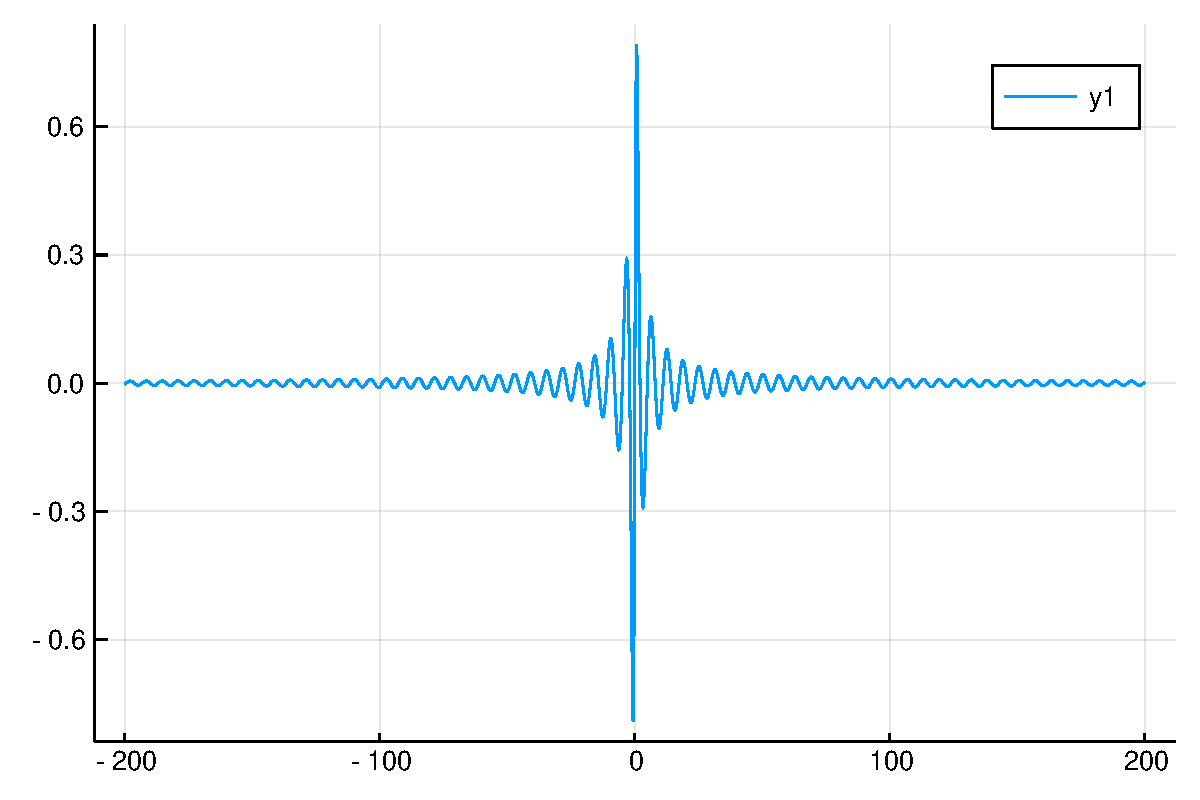
\includegraphics[width=\linewidth]{figures/Lecture5_9_1.pdf}

An equivalent result holds in the negative real axis, but be careful:


\begin{lstlisting}
(*@\HLJLn{z}@*) (*@\HLJLoB{=}@*) (*@\HLJLoB{-}@*)(*@\HLJLni{2}@*)(*@\HLJLoB{-}@*)(*@\HLJLn{im}@*)
(*@\HLJLn{f}@*) (*@\HLJLoB{=}@*) (*@\HLJLn{x}@*) (*@\HLJLoB{->}@*) (*@\HLJLnf{exp}@*)(*@\HLJLp{(}@*)(*@\HLJLn{im}@*)(*@\HLJLoB{*}@*)(*@\HLJLn{x}@*)(*@\HLJLp{)}@*)(*@\HLJLoB{/}@*)(*@\HLJLp{(}@*)(*@\HLJLn{x}@*)(*@\HLJLoB{+}@*)(*@\HLJLn{im}@*)(*@\HLJLp{)}@*)
(*@\HLJLnf{sum}@*)(*@\HLJLp{(}@*)(*@\HLJLnf{Fun}@*)(*@\HLJLp{(}@*)(*@\HLJLn{x}@*)(*@\HLJLoB{->}@*) (*@\HLJLnf{f}@*)(*@\HLJLp{(}@*)(*@\HLJLn{x}@*)(*@\HLJLp{)}@*)(*@\HLJLoB{/}@*)(*@\HLJLp{(}@*)(*@\HLJLn{x}@*) (*@\HLJLoB{-}@*) (*@\HLJLn{z}@*)(*@\HLJLp{),}@*) (*@\HLJLoB{-}@*)(*@\HLJLni{500}@*) (*@\HLJLoB{..}@*) (*@\HLJLni{500}@*)(*@\HLJLp{))}@*)(*@\HLJLoB{/}@*)(*@\HLJLp{(}@*)(*@\HLJLni{2}@*)(*@\HLJLn{\ensuremath{\pi}}@*)(*@\HLJLoB{*}@*)(*@\HLJLn{im}@*)(*@\HLJLp{)}@*)
\end{lstlisting}

\begin{lstlisting}
-4.529525111429054e-9 + 5.865568293152012e-7im
\end{lstlisting}


\begin{lstlisting}
(*@\HLJLn{z}@*) (*@\HLJLoB{=}@*) (*@\HLJLoB{-}@*)(*@\HLJLni{2}@*)(*@\HLJLoB{-}@*)(*@\HLJLn{im}@*)
(*@\HLJLn{f}@*) (*@\HLJLoB{=}@*) (*@\HLJLn{x}@*) (*@\HLJLoB{->}@*) (*@\HLJLnf{exp}@*)(*@\HLJLp{(}@*)(*@\HLJLn{im}@*)(*@\HLJLoB{*}@*)(*@\HLJLn{x}@*)(*@\HLJLp{)}@*)(*@\HLJLoB{/}@*)(*@\HLJLp{(}@*)(*@\HLJLn{x}@*)(*@\HLJLoB{-}@*)(*@\HLJLn{im}@*)(*@\HLJLp{)}@*)
(*@\HLJLnf{sum}@*)(*@\HLJLp{(}@*)(*@\HLJLnf{Fun}@*)(*@\HLJLp{(}@*)(*@\HLJLn{x}@*)(*@\HLJLoB{->}@*) (*@\HLJLnf{f}@*)(*@\HLJLp{(}@*)(*@\HLJLn{x}@*)(*@\HLJLp{)}@*)(*@\HLJLoB{/}@*)(*@\HLJLp{(}@*)(*@\HLJLn{x}@*) (*@\HLJLoB{-}@*) (*@\HLJLn{z}@*)(*@\HLJLp{),}@*) (*@\HLJLoB{-}@*)(*@\HLJLni{500}@*) (*@\HLJLoB{..}@*) (*@\HLJLni{500}@*)(*@\HLJLp{))}@*)(*@\HLJLoB{/}@*)(*@\HLJLp{(}@*)(*@\HLJLni{2}@*)(*@\HLJLn{\ensuremath{\pi}}@*)(*@\HLJLoB{*}@*)(*@\HLJLn{im}@*)(*@\HLJLp{),}@*) (*@\HLJLnf{f}@*)(*@\HLJLp{(}@*)(*@\HLJLn{z}@*)(*@\HLJLp{)}@*)
\end{lstlisting}

\begin{lstlisting}
(0.09196985577264773 - 0.09196926921581833im, 0.9007327639404081 + 0.335130
5720620013im)
\end{lstlisting}


\begin{lstlisting}
(*@\HLJLn{z}@*) (*@\HLJLoB{=}@*) (*@\HLJLoB{-}@*)(*@\HLJLni{2}@*)(*@\HLJLoB{-}@*)(*@\HLJLn{im}@*)
(*@\HLJLn{f}@*) (*@\HLJLoB{=}@*) (*@\HLJLn{x}@*) (*@\HLJLoB{->}@*) (*@\HLJLnf{exp}@*)(*@\HLJLp{(}@*)(*@\HLJLoB{-}@*)(*@\HLJLn{im}@*)(*@\HLJLoB{*}@*)(*@\HLJLn{x}@*)(*@\HLJLp{)}@*)(*@\HLJLoB{/}@*)(*@\HLJLp{(}@*)(*@\HLJLn{x}@*)(*@\HLJLoB{-}@*)(*@\HLJLn{im}@*)(*@\HLJLp{)}@*)
(*@\HLJLoB{-}@*)(*@\HLJLnf{sum}@*)(*@\HLJLp{(}@*)(*@\HLJLnf{Fun}@*)(*@\HLJLp{(}@*)(*@\HLJLn{x}@*)(*@\HLJLoB{->}@*) (*@\HLJLnf{f}@*)(*@\HLJLp{(}@*)(*@\HLJLn{x}@*)(*@\HLJLp{)}@*)(*@\HLJLoB{/}@*)(*@\HLJLp{(}@*)(*@\HLJLn{x}@*) (*@\HLJLoB{-}@*) (*@\HLJLn{z}@*)(*@\HLJLp{),}@*) (*@\HLJLoB{-}@*)(*@\HLJLni{500}@*) (*@\HLJLoB{..}@*) (*@\HLJLni{500}@*)(*@\HLJLp{))}@*)(*@\HLJLoB{/}@*)(*@\HLJLp{(}@*)(*@\HLJLni{2}@*)(*@\HLJLn{\ensuremath{\pi}}@*)(*@\HLJLoB{*}@*)(*@\HLJLn{im}@*)(*@\HLJLp{),}@*) (*@\HLJLnf{f}@*)(*@\HLJLp{(}@*)(*@\HLJLn{z}@*)(*@\HLJLp{)}@*)
\end{lstlisting}

\begin{lstlisting}
(-0.045354995402086956 - 0.1219015148055592im, -0.04535499089125899 - 0.121
90092372837213im)
\end{lstlisting}


\subsubsection{Fourier transforms and Jordan's lemma}
The case of calculating

\[
    \int_{-\infty}^\infty e^{\I \omega x} g(x) dx
\]
is important because it is the Fourier transform of $g(x)$. Provided $g$ is defined in the upper half plane and $\omega > 0$,  $f(z) = e^{\I \omega z} g(z)$  has exponential decay. If $g$ decays fast enough we can use residue calculus as before. 

\textbf{Example} Consider the Fourier transform of $g(x) = 1/(x^2+1)$. This decays fast enough to use residue calculus so we have for $\omega > 0$

\[
\int_{-\infty}^\infty {\E^{\I \omega x } \over x^2 + 1} \D x = 2 \pi \I \Res_{z = \I} {\E^{\I \omega z } \over z^2 + 1} = \pi \E^{-\omega}.
\]
On the other hand if $\omega < 0$ we have exponential decay in lower half plane and use corresponding residues to determine

\[
\int_{-\infty}^\infty {\E^{\I \omega x } \over x^2 + 1} \D x = -2 \pi \I \Res_{z = -\I} {\E^{\I \omega z } \over z^2 + 1} = \pi \E^{\omega}.
\]
That is, the Fourier transform of $g(x) = 1/(x^2+1)$ is $\pi \E^{-|\omega|}$. 

Exponential decay actually gives us  sharper results:

\textbf{Lemma (Jordan)} Assume $\omega > 0$. If $g(z)$ is continuous in on the half circle $H_R = \{ R e^{i \theta} : 0 \leq \theta \leq \pi \}$  then

\[
\left| \int_{H_R} g(z) e^{\I \omega z} dz \right| \leq {\pi \over \omega} M
\]
where $M = \sup_{z \in H_R} |g(z)|$. 

\textbf{Sketch of proof} We have

\[
\left| \int_{H_R} g(z) e^{\I \omega z} dz \right|  \leq   R \int_0^\pi \left|g(R e^{i \theta}) e^{\I \omega R e^{i \theta}}e^{i \theta}\right| d\theta 
\leq MR \int_0^\pi e^{- \omega R\sin \theta } d\theta 
= 2MR \int_0^{\pi\over 2} e^{- \omega R\sin \theta } d\theta 
\]
But we have $\sin \theta \geq {2 \theta \over \pi}$:


\begin{lstlisting}
(*@\HLJLn{\ensuremath{\theta}}@*) (*@\HLJLoB{=}@*) (*@\HLJLnf{range}@*)(*@\HLJLp{(}@*)(*@\HLJLni{0}@*)(*@\HLJLp{;}@*) (*@\HLJLn{stop}@*)(*@\HLJLoB{=}@*)(*@\HLJLn{\ensuremath{\pi}}@*)(*@\HLJLoB{/}@*)(*@\HLJLni{2}@*)(*@\HLJLp{,}@*) (*@\HLJLn{length}@*)(*@\HLJLoB{=}@*)(*@\HLJLni{100}@*)(*@\HLJLp{)}@*)
(*@\HLJLnf{plot}@*)(*@\HLJLp{(}@*)(*@\HLJLn{\ensuremath{\theta}}@*)(*@\HLJLp{,}@*) (*@\HLJLn{sin}@*)(*@\HLJLoB{.}@*)(*@\HLJLp{(}@*)(*@\HLJLn{\ensuremath{\theta}}@*)(*@\HLJLp{);}@*) (*@\HLJLn{label}@*)(*@\HLJLoB{=}@*)(*@\HLJLs{"{}sin}@*) (*@\HLJLs{t"{}}@*)(*@\HLJLp{)}@*)
(*@\HLJLnf{plot!}@*)(*@\HLJLp{(}@*)(*@\HLJLn{\ensuremath{\theta}}@*)(*@\HLJLp{,}@*) (*@\HLJLni{2}@*)(*@\HLJLn{\ensuremath{\theta}}@*)(*@\HLJLoB{/}@*)(*@\HLJLn{\ensuremath{\pi}}@*)(*@\HLJLp{;}@*) (*@\HLJLn{label}@*) (*@\HLJLoB{=}@*) (*@\HLJLs{"{}2t}@*) (*@\HLJLs{/}@*) (*@\HLJLs{pi"{}}@*)(*@\HLJLp{)}@*)
\end{lstlisting}

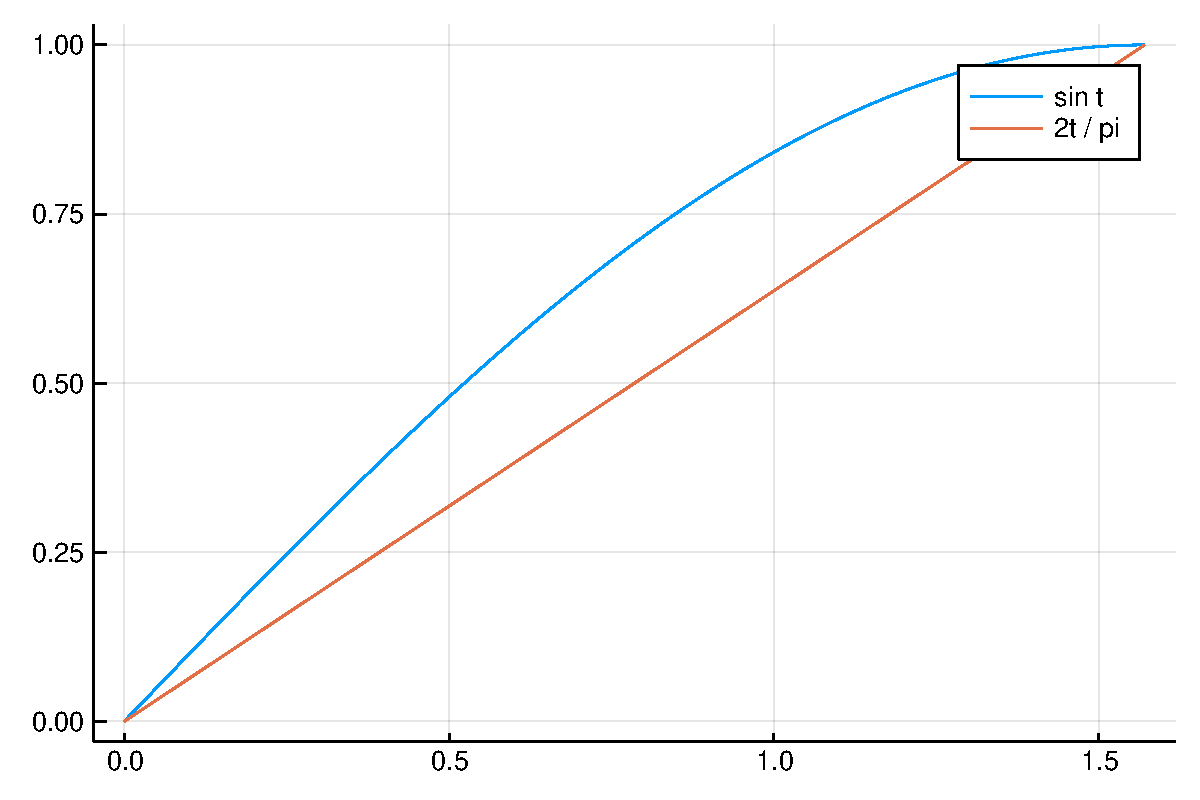
\includegraphics[width=\linewidth]{figures/Lecture5_13_1.pdf}

Hence 

\[
\left| \int_{H_R} g(z) e^{\I \omega z} dz \right|  \leq  2MR \int_0^{\pi\over 2} e^{- {2\omega R\theta \over \pi} } d\theta = {\pi \over \omega} (1 - e^{-\omega R}) M \leq {\pi M \over \omega}.
\]
\subsection{Application: Calculating Fourier integrals of weakly decaying functions}
Why is this useful? We can use it to apply Residue theorem to  functions that only have $z^{-1}$ decay. Such functions do not decay absolutely but do  converge in a principal value sense: 


\begin{lstlisting}
(*@\HLJLn{f}@*) (*@\HLJLoB{=}@*) (*@\HLJLn{x}@*) (*@\HLJLoB{->}@*) (*@\HLJLnf{exp}@*)(*@\HLJLp{(}@*)(*@\HLJLn{im}@*)(*@\HLJLoB{*}@*)(*@\HLJLn{x}@*)(*@\HLJLp{)}@*)(*@\HLJLoB{*}@*)(*@\HLJLn{x}@*)(*@\HLJLoB{/}@*)(*@\HLJLp{(}@*)(*@\HLJLn{x}@*)(*@\HLJLoB{{\textasciicircum}}@*)(*@\HLJLni{2}@*)(*@\HLJLoB{+}@*)(*@\HLJLni{1}@*)(*@\HLJLp{)}@*)

(*@\HLJLnf{sum}@*)(*@\HLJLp{(}@*)(*@\HLJLnf{Fun}@*)(*@\HLJLp{(}@*)(*@\HLJLn{f}@*)(*@\HLJLp{,}@*) (*@\HLJLoB{-}@*)(*@\HLJLni{30000}@*) (*@\HLJLoB{..}@*) (*@\HLJLni{30000}@*)(*@\HLJLp{))}@*)
\end{lstlisting}

\begin{lstlisting}
-6.776263578034403e-21 + 1.1557671135433842im
\end{lstlisting}


Thus we can construct a Residue theorem for calculating 

\[
\infdashint g(x) e^{\I \omega x} \dx
\]
provided that $g(z) \rightarrow 0$ and is analytic in the upper-half plane.


\begin{lstlisting}
(*@\HLJLni{2}@*)(*@\HLJLn{\ensuremath{\pi}}@*)(*@\HLJLoB{*}@*)(*@\HLJLn{im}@*)(*@\HLJLoB{*}@*)(*@\HLJLnf{exp}@*)(*@\HLJLp{(}@*)(*@\HLJLoB{-}@*)(*@\HLJLni{1}@*)(*@\HLJLp{)}@*)(*@\HLJLoB{*}@*)(*@\HLJLn{im}@*)(*@\HLJLoB{/}@*)(*@\HLJLp{(}@*)(*@\HLJLn{im}@*)(*@\HLJLoB{+}@*)(*@\HLJLn{im}@*)(*@\HLJLp{)}@*)  (*@\HLJLcs{{\#}}@*) (*@\HLJLcs{2\ensuremath{\pi}*im*}@*) (*@\HLJLcs{residue}@*) (*@\HLJLcs{of}@*) (*@\HLJLcs{g(z)exp(im*z)}@*) (*@\HLJLcs{at}@*) (*@\HLJLcs{z}@*) (*@\HLJLcs{=}@*) (*@\HLJLcs{im}@*)
\end{lstlisting}

\begin{lstlisting}
0.0 + 1.1557273497909217im
\end{lstlisting}



\end{document}
